\section{Window Layout Concept}
    Developers can define their working environment to fit the needs and preferences. For a better understanding of
    further comments and instructions, lets define five major areas of the main window.

   \begin{figure}[h]
        \centering
        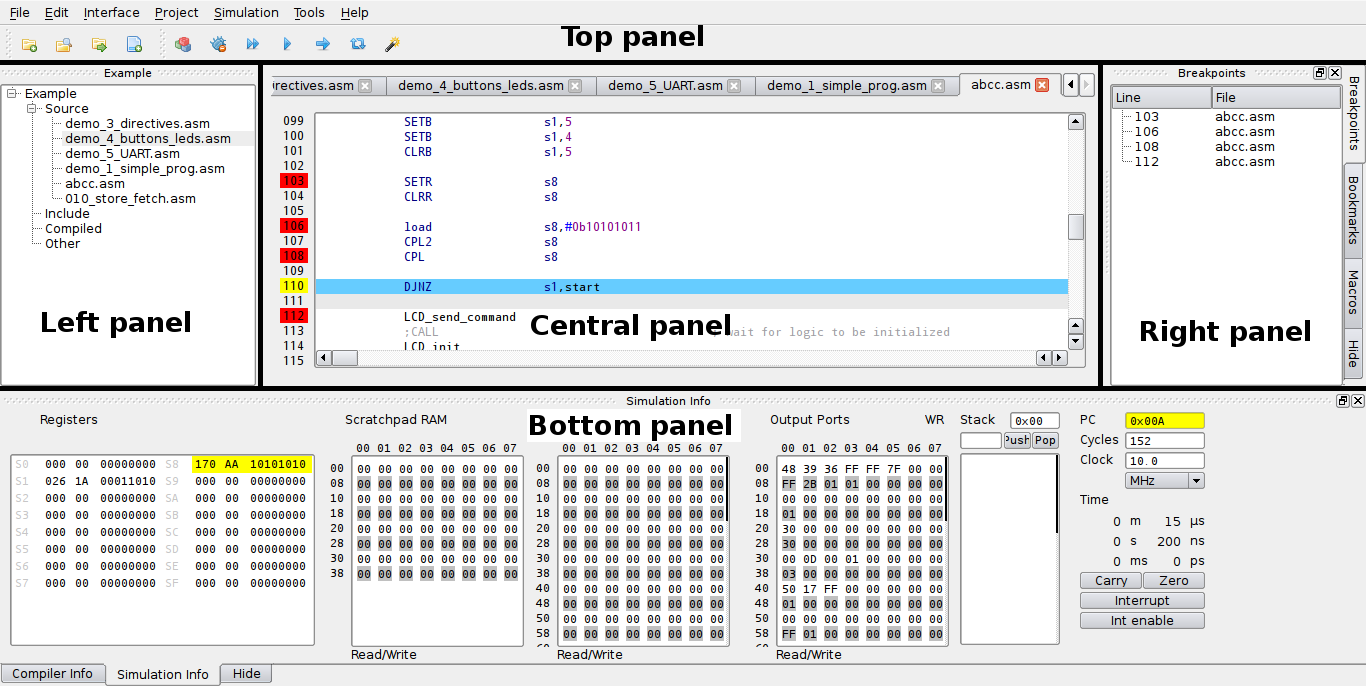
\includegraphics[width=\textwidth]{img/Main_window.png}
        \caption{Window layout concept}
    \end{figure}

    \subsection{Central panel}
        Central panel contains the main text editor with syntax highlight for writing a source code. In the editor you can
        also easily add breakpoints and bookmarks just by clicking on desired line number by left or right mouse button,
        each invokes different action.

    \subsection{Top panel}
    \begin{figure}[h!]
            \centering
            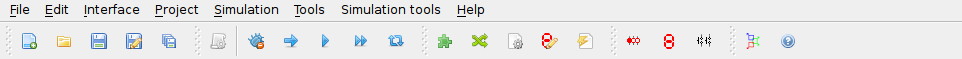
\includegraphics[width=0.75\textwidth]{img/top_panel.png}
            \caption{Toolbar icons}
        \end{figure}

    \subsubsection{Top panel icons}
        \begin{itemize}
            \item New project: Creates a new project.
            \item Open project: Opens an existing project file.
            \item Save project: Saves current project file.
            \item Compile: Compiles your code.
            \item Start Simulation: Enters simulation mode.
            \item Run: High speed simulation.
            \item Animate: Simulation with GUI (such as register view, etc.) updated after each executed instruction.
            \item Step: Step by step simulation.
            \item Reset: Resets simulator to its initial state.
            \item Unhighlight: Clear highlight from register view and other graphical components of the simulator panel.
            \item Undo: will undo all edit actions on the open document in reverse order
            \item Redo: will redo all undo actions
            \item Cut: cuts all selected parts of the open document and puts it in the clipboard.
            \item Copy: copies all selected parts of the open document to the clipboard
            \item Paste: pastes the text contents of the clipboard in the open document
            \item Select: All selects all text in the open document
            \item Find: find a to be given string through the open document
            \item Replace: replace a given string in the open document by a new string
        \end{itemize}

    \subsection{Bottom panel}
        Bottom panel consists of simulator main panel, and compiler messages.

        In simulator main panel you can see status of internal registers, scratch-pad ram, input and output ports, call
        stack, program counter, elapsed time and machine cycles, processor clock, and internal flags carry and zero. All
        these values can be edited during processor simulation.

        In compiler messages panel you can see textual output from the assembler, like warnings and other messages.

        \begin{figure}[h!]
            \centering
            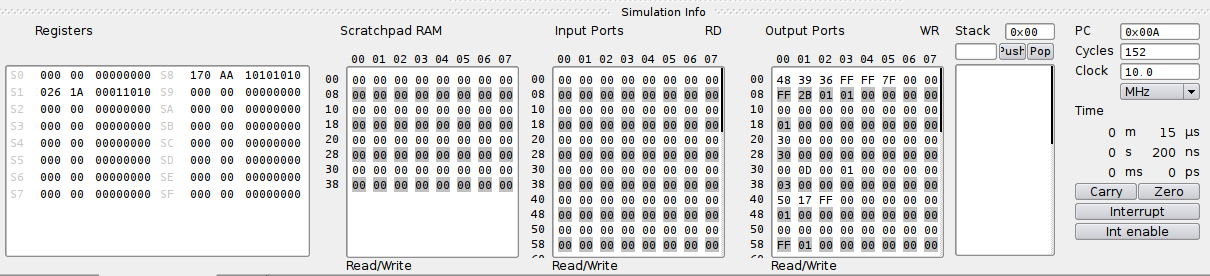
\includegraphics[width=\textwidth]{img/bottom_panel.png}
            \caption{Bottom panel}
        \end{figure}

    \subsection{Left panel}
        Here you can see main project tree. You can close or configure project by right clicking on the project name, add a
        file to the project or create a new one. You can also see included files or opened compiled files like .lst, etc.

    \subsection{Right panel}
        Right panel contains lists of breakpoints, bookmarks, symbols, and macros in your source code.

        \begin{table}[h!]
            \begin{tabular}{cc}
                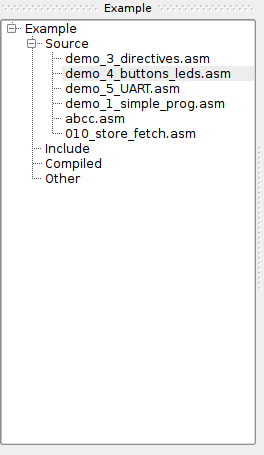
\includegraphics[width=.33\textwidth]{img/left_panel.png}
                    &
                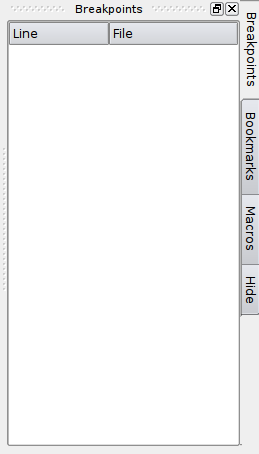
\includegraphics[width=.33\textwidth]{img/right_panel.png}
                    \\
                Left panel & Right panel
            \end{tabular}
        \end{table}

\clearpage

\section{Project configuration}
    In project configuration window, you can edit project and compiler settings. You can open project configuration
    window by right clicking on project name in the left panel and choosing Configuration, see the pictures below.
    This will open main configuration window with multiple tabs on the left side.

    \subsubsection{Project - Options}
        \begin{itemize}
            \item Project name: Name of your project.
            \item Architecture: Processor architecture for your project.
            \item Family: Processor family of the selected architecture.
            \item Info panel: Brief description of selected processor.
        \end{itemize}

        \subsubsection{Project - Memory}
            \begin{itemize}
                \item Size options: Tell the compiler your processor's memory size.
                \item Interrupt vector: Set your interrupt vector (size of program memory - 1 is maximum),
                \item HW build: Your HW build constant.
            \end{itemize}

        \begin{table}[h!]
            \begin{tabular}{cc}
                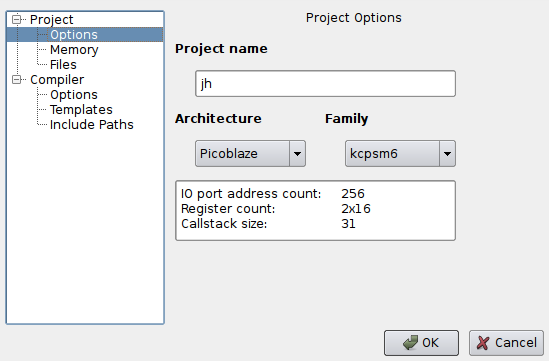
\includegraphics[width=.5\textwidth]{img/config2.png}
                    &
                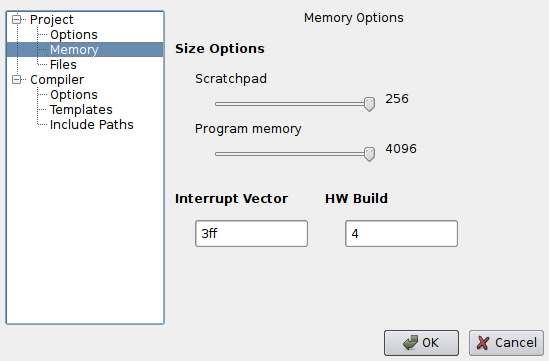
\includegraphics[width=.5\textwidth]{img/config1.png}
                    \\
                Project - Options & Project - Memory
            \end{tabular}
        \end{table}

    \subsubsection{Project - Files}
        Here is where you can create, add, or remove files from your project, and set set the main file (see below).

    \clearpage

    \subsubsection{Compiler - Options}
            \begin{itemize}
                \item Main file: If you have "Use main file" checked, you can choose which file will always chosen for
                      compilation and simulation instead of the file current opened in the editor.
                \item Generate: Select which files should the assembler generate in your project's directory from the
                      given source code.
            \end{itemize}

        \begin{table}[h!]
            \begin{tabular}{cc}
                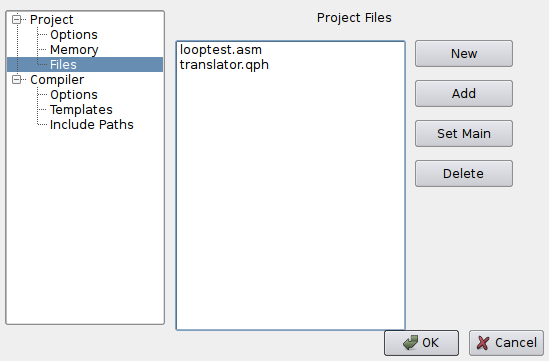
\includegraphics[width=.5\textwidth]{img/config3.png}
                    &
                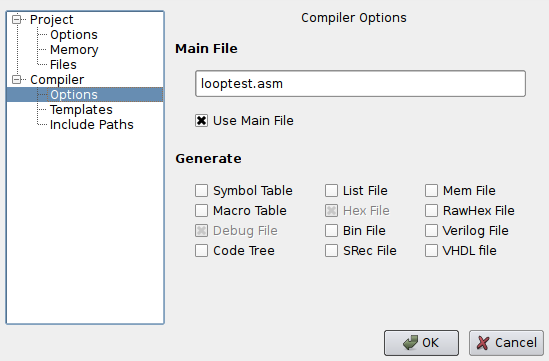
\includegraphics[width=.5\textwidth]{img/config4.png}
                    \\
                Project - Files & Compiler - Options
            \end{tabular}
        \end{table}

        \subsubsection{Compiler - templates}
            Choose which VHDL or Verilog template will be used by the assembler to generate the HDL code for your
            design, by default MDS uses its own built-in templates.

        \subsubsection{Compiler - include paths}
            Here you can add or edit path, where the compiler will try to find files included in other source code files
            (directive INCLUDE).

        \begin{table}[h!]
            \begin{tabular}{cc}
                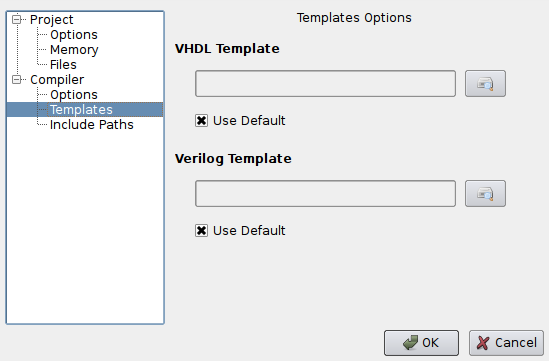
\includegraphics[width=.5\textwidth]{img/config5.png}
                    &
                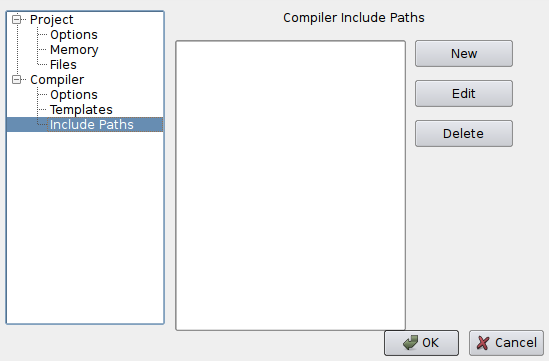
\includegraphics[width=.5\textwidth]{img/config6.png}
                    \\
                Compiler - Templates & Compiler - Include paths
            \end{tabular}
            \end{table}

\section{Interface configuration}
    In interface configuration dialog, you can edit IDE behavior and appearance, for instance editor font, tab width,
    etc., or simulator warnings. To open the interface configuration dialog, click on [Main~Menu] -> [Interface] ->
    [Config].

    \subsubsection{IDE - General}
        In the general settings you can set if you want splash screen, session restoration, or change language of whole
        IDE (this option is available only when language pack for your language is available.).

    \subsubsection{Editor - General}
        General settings of IDE editor. You can set tab width, number of spaces .

        \begin{table}[h!]
            \begin{tabular}{cc}
                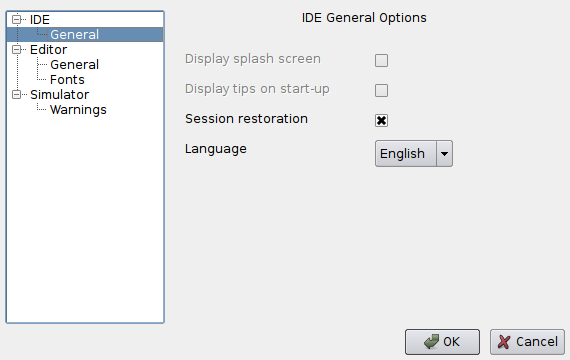
\includegraphics[width=.5\textwidth]{img/interface1.png}
                    &
                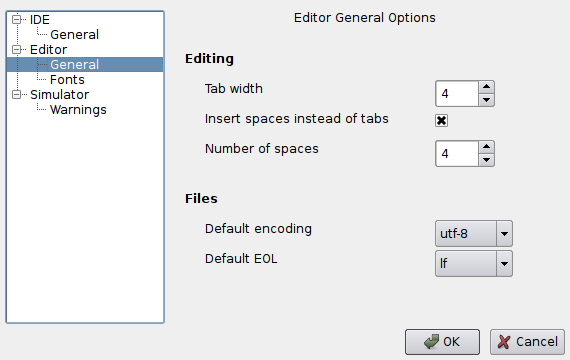
\includegraphics[width=.5\textwidth]{img/interface2.png}
                    \\
                IDE - General & Editor - General
            \end{tabular}
        \end{table}

        \begin{table}[h!]
            \begin{tabular}{cc}
                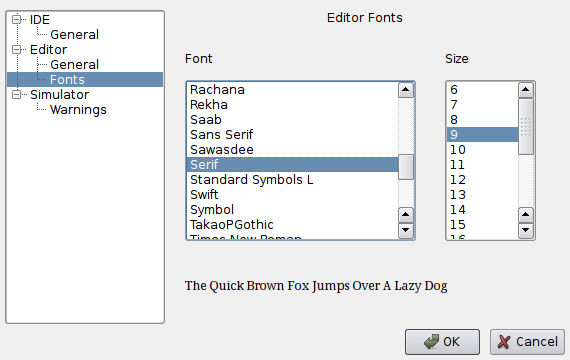
\includegraphics[width=.5\textwidth]{img/interface3.png}
                    &
                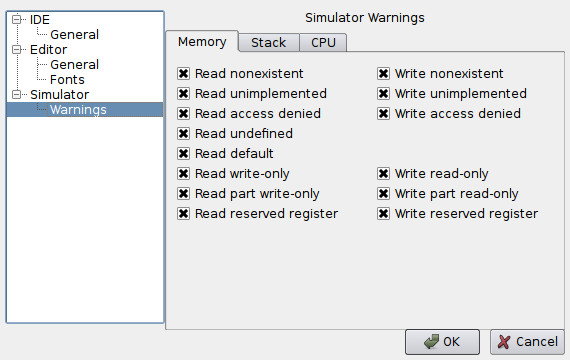
\includegraphics[width=.5\textwidth]{img/interface4.png}
                    \\
                Editor - Fonts & Simulator - Warnings -> Memory
            \end{tabular}
        \end{table}

        \begin{table}[h!]
            \begin{tabular}{cc}
                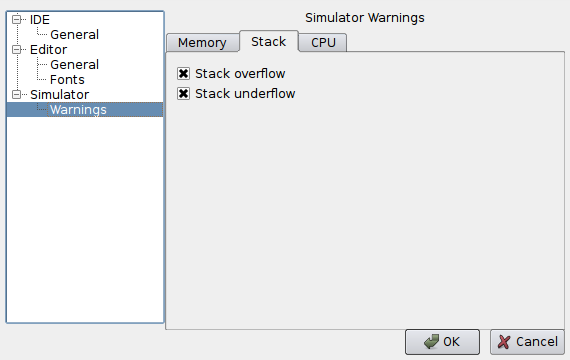
\includegraphics[width=.5\textwidth]{img/interface5.png}
                    &
                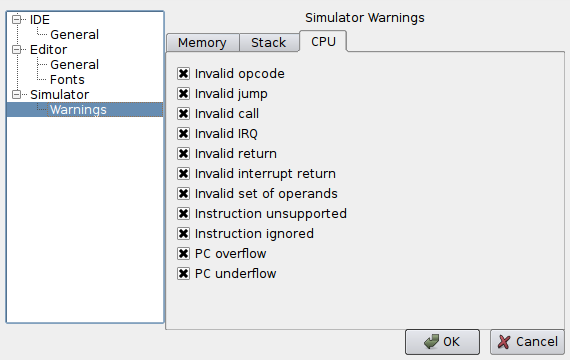
\includegraphics[width=.5\textwidth]{img/interface6.png}
                    \\
                Simulator - Warnings -> Stack & Simulator - Warnings -> CPU
            \end{tabular}
        \end{table}

\section{Data file converter}
    This tool allows you to convert selected data file to another. Mutual conversion can be made between .ihex, .bin,
    .srec, .mem, .rawhex, .v, and .vhd.
    \begin{description}
        \item[Section Input File] Here you can select desired input data file which will be converted.
        \item[Section Input Options] In this section, you define what type of input file will be converted.
        \item[Input file type] Available options - Hex, Bin, SRec, XilMem, XilVerilog and XilVhdl.
        \item[Bytes per record] Only if you want to convert XilMem file. Defines number of bytes per record.
        \item[OPCode size] Defines opcode size of selected data file. Available are 16 and 18.
        \item[Section Output File] Defines target.
        \item[Section Output Options] Here you can select desired output data file.
        \item[Input file type] Available options - Hex, Bin, SRec, XilMem, XilVerilog and XilVhdl.
        \item[Tab size]  Define number of inserted spaces when you press Tab.
        \item[Short instructions] Here you can allow short instructions like LD, RETI, etc.
    \end{description}

    \begin{figure}[h]
        \centering{}
        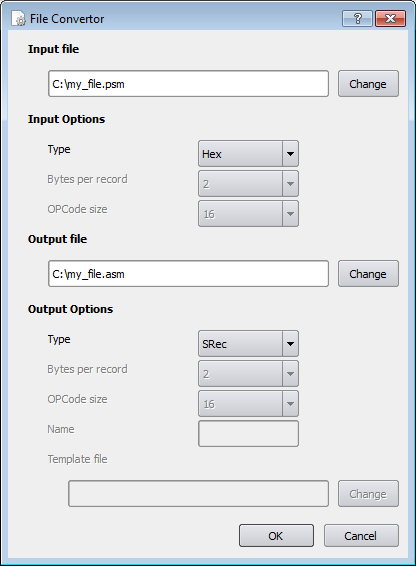
\includegraphics[width=.5\textwidth]{img/DATA_converter.png}
        \caption{DATA file converter}
    \end{figure}

\section{Assembler translator}
    With this tool, you can translate your previously written assembler code in different syntax.
    You can select one of three choices - Xilinx, Mediatronix and OpenPicIde. Input code has to be without
    errors.
    \begin{description}
        \item[Section Input File] Here you can choose which file you want to translate into the MDS assembler
        \item[Section ASM type] Input file syntax version. Translator needs to know input file syntax. Select one of
             three choices - Xilinx, Mediatronix and OpenPicIde.
        \item[Symbol] Case of symbols - uppercase or lowercase
        \item[End of line] Indentation - Choose between Tabs or Spaces
        \item[Directive] Case of Directives - uppercase or lowercase
        \item[Indentation] Three choices - Tabs, Spaces and Keep (indentation unchanged)
        \item[Instruction] Case of instructions - uppercase or lowercase
        \item[Tab size]  Define number of inserted spaces when you press Tab.
        \item[Short instructions] Here you can allow short instructions like LD, RETI or others
    \end{description}

    \begin{figure}[h]
        \centering{}
        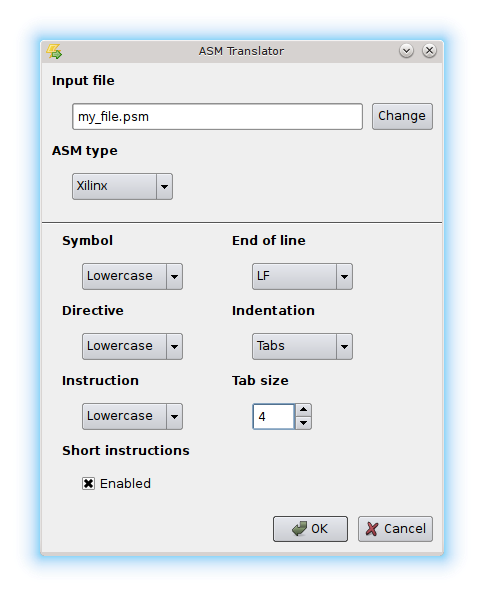
\includegraphics[width=.5\textwidth]{img/ASM_translator.png}
        \caption{ASM translator}
    \end{figure}

\section{Disassembler}
    Disassembler is a tool that translates machine language into assembly language. The inverse
    operation to that of an assembler.

    \begin{description}
        \item[Section File] Choose which file you want to disassemble.
        \item[Section Target] Your processor architecture
        \item[Family] Processor family of the selected architecture.
        \item[Indentation] Choose between tabs and spaces.
        \item[Tab size] Tab size measured in number of spaces.
        \item[Radix] Binary, octal, decimal, or hexadecimal.
        \item[Line break] CRLF (Windows), LF (Linux), or CR (Mac)
        \item[Case] Use upper case or lower case characters.
        \item[Generate symbols] Which symbols should be named.
    \end{description}

    \begin{figure}[h]
        \centering{}
        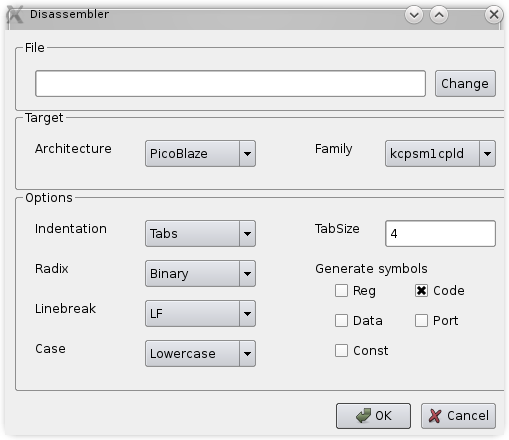
\includegraphics[width=.5\textwidth]{img/disassembler_window.png}
        \caption{Disassembler}
    \end{figure}

\section{Delay loop generator}
    In many cases, it is useful to have a tool for creating delay loops, it can just save you some time in the
    development process. This tool can generate wait loops using up to six registers as iterators. All you have to do is
    enter desired time of delay or number of cycles and clock frequency.

    \begin{description}
        \item[Section Input variable] Choose between time or cycles
        \item[Section Desired waiting time] Number of executed time or cycles
        \item[Section Frequency] Clock frequency
        \item[Section Register names] Set register names used in the generated code (optional).
        \item[Section Generated code] The generated code.
        \item[Instruction] Instruction used in loop.
        \item[Type] Type of waiting loop you want to create (blank/macro).
        \item[Upper Case and Comments]  Turn off automatically added comments, and use upper case.
        \item[Button Copy to clipboard] This will copy the generated code to clipboard.
        \item[Button Generate] Generate code.
    \end{description}

    \begin{figure}[h]
        \centering{}
        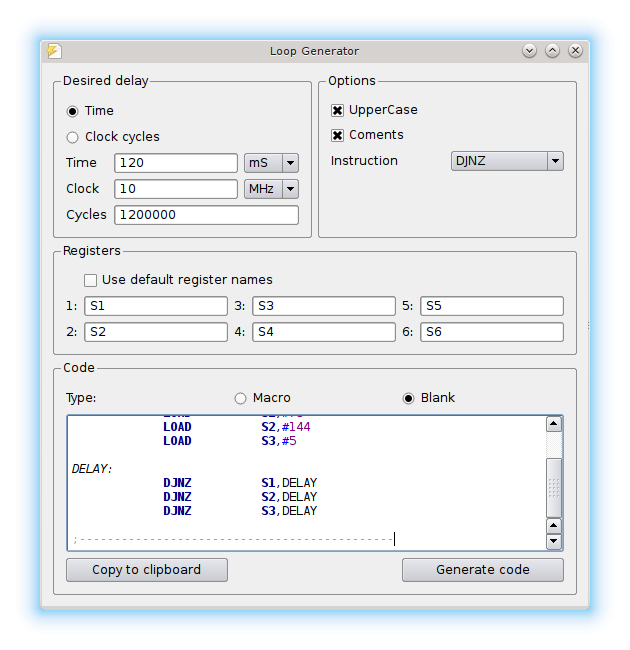
\includegraphics[width=.7\textwidth]{img/loop_gen.png}
        \caption{Delay loop generator dialog}
    \end{figure}

\section{8-segment editor}
    \begin{wrapfigure}{r}{0pt}
        \centering{}
        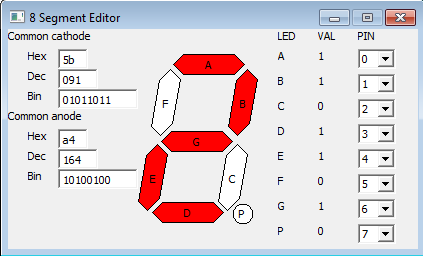
\includegraphics[width=110pt]{img/8segment.png}
        \caption{8-segment editor}
    \end{wrapfigure}
    With this tool you can easily determine what value you have to set on a port to display a digit on a numerical LED
    display. In the left part of the dialog window, you can find numerical values corresponding to the displayed digit
    in the middle part. These values are represented for both common cathode and common anode and in three numerical
    bases: hexadecimal, decimal, and octal. Buttons on left side from entry boxes copies value from the adjacent entry
    box to clipboard. In the right part of the window you can set what port pin is connected to what LED segment, this
    sets permutation of the resulting value(s).

\section{LED panel simulator}
    \begin{wrapfigure}{r}{0pt}
        \centering{}
        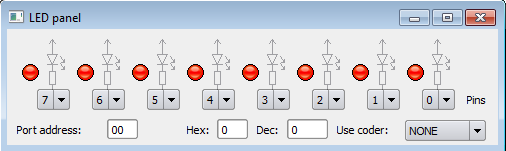
\includegraphics[width=150pt]{img/Led_panel.png}
        \caption{8-segment editor}
    \end{wrapfigure}

    Simple LED panel simulator. You can observe output port behavior with visual representation of eight LEDs. You can
    set BCD and Gray decoder to simulate common FPGA logic.

    \begin{description}
        \item[GRAY] Converts output port value to gray code.
        \item[BCD] Output port value will be presented as BCD. Remember that bigger number than 99 cannot be displayed.
    \end{description}

\section{7-segment simulator}
    \begin{wrapfigure}{r}{0pt}
        \centering{}
        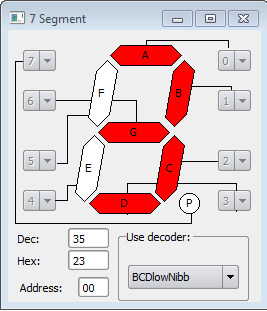
\includegraphics[width=110pt]{img/7seg_sim.png}
        \caption{7-segment simulator}
    \end{wrapfigure}
    Simulator of 7-segment display with common anode, the display is connected to an output port. Port bits can be
    assigned to any display segment. Multiple instances of this simulator can be opened at once. You can set BCD decoder
    to simulate commonly used FPGA logic.

    \begin{description}
        \item[BCDlowNibb] Low-order nibble is decoded and displayed.
        \item[BCDhighNibb] High-order nibble is decoded and displayed.
    \end{description}

\section{Number base converter}
    \begin{wrapfigure}{r}{0pt}
            \centering
            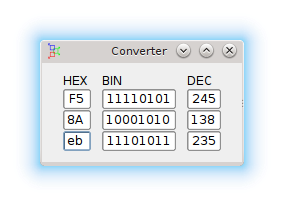
\includegraphics[width=90pt]{img/converter.png}
            \caption{Converter}
    \end{wrapfigure}

    This tool is very useful when you want to quickly convert some number to another radix.
